\documentclass{article}
\usepackage[utf8]{inputenc}
\usepackage{geometry}
\usepackage{graphicx}
\geometry{margin = .25in}
\usepackage{amsmath, amsthm, amssymb, enumitem}
\usepackage{etoolbox}
\newtheorem{problem}{Problem}
\theoremstyle{definition}
\newtheorem*{solution}{Solution}

\begin{document}

\title{Math 240 (Discrete Structures 1) Assignment 8}
\author{Victoria Pittard, ID 260762268}
\date{\today}

\maketitle

%Problem 1
\begin{problem}\textbf{Principle of Inclusion-Exclusion.}
\begin{enumerate}[label = \alph*)]
    \item Determine the number of integers from 1 to 1,000,000 which are relatively prime to 990,099.
    
    \item Out of a group of 30 people, 20 people play the flute, 8 play piano, and 25 play violin. If 20 people play at least two of the three instruments and 6 play all three, how many of the 30 people play none of the three instruments?
\end{enumerate}
\end{problem}

\begin{solution}
\end{solution}
\begin{enumerate}[label = \alph*)]
    \item There are 1,000,000 total options, and the prime factors of 990,099 are 3, 11, 73, and 137. According to the principle of inclusion-exclusion, to find the number of values in the range not divisible by any of these, you have to subtract the values divisible by one of the prime factors, add the values divisible by two of the prime factors, subtract the values divisible by three of the prime factors, and finally add the values divisible by all of the prime factors. This gives you $1,000,000 - [\frac{1000000}{3} + \frac{1000000}{11} + \frac{1000000}{73} + \frac{1000000}{137}] + [\frac{1000000}{3*11}+\frac{1000000}{3*73}+\frac{1000000}{3*137}+\frac{1000000}{11*73}+\frac{1000000}{11*137}+\frac{1000000}{73*137}] - [\frac{1000000}{3*11*73}+\frac{1000000}{3*11*137}+\frac{1000000}{3*73*37}+\frac{1000000}{11*73*37}]+[\frac{1000000}{3*11*73*137}]$, or 593395.
    
    \item By principle of inclusion-exclusion, you must add the people who play each individual instrument, subtract those who play at least two, and then subtract again those who play all three to find the number of people who play an instrument. Then, subtract this from 30. This gives you $30-[(20+8+25)-(20-6)-(2*6)]$, or 3.
\end{enumerate}

%Problem 2
\begin{problem}\textbf{Pigeon Hole Principle.}
\begin{enumerate}[label = \alph*)]
    \item Let X be a subset of the integers from 1 to 1997 such that $|X|\ge 34$. Show that there exist distinct $a, b, c \in X$ and distinct $x,y,z\in X$ such that $a+b+c=x+y+z$ and $\{ a,b,c \} \neq \{x,y,z\}$.
    
    \item Let $n$ be any positive integer, and let $d$ be a positive integer such that $1\le d \le 9$. Show that some multiple of $n$ can be expressed in base 10 using only the digits 0 and $d$.
\end{enumerate}
\end{problem}

\begin{solution}
\end{solution}
\begin{enumerate}[label = \alph*)]
    \item $A = \{x\in \mathbb{Z} | 1\le x \le 1997\}$, and X is a subset of A with at least 34 elements. Regardless of X, the largest possible sum of three numbers in X is 1995+1996+1997, or 5988. The lowest possible sum of three numbers in X is 1+2+3, or 6. 5988-6+1 (one is added as the two extremes are both included) is equal to 5983 possible sums. X must have at least 34 elements, and $\binom{34}{3}$ = $\frac{34!}{3!31!}$ = 5984. By the pigeon hole principle, if you have 5983 "holes" (possible distinct sums) and 5984 "pigeons" (sums of three values in the subset), two of the pigeons must be in the same whole (equal sum, obtained by adding different values).
    
    \item If you consider the set $M=\{M_1, ... , M_{n+1}\}$, where $M_i$ is a number with i digits, each of which is d, and divide all the values of set M by n, there are always at least two values that have the same remainder (equivalent mod n). For example, if n=3 and d=7, $M_1$ and $M_4$ both are equivalent to 1 mod 3. Thus, through the pigeon hole principle, as there are n+1 values in the set, and n remainders, there must be two numbers with the same remainder.
\end{enumerate}

%Problem 3
\begin{problem}\textbf{Graphs.} For each of the following degree sequences, either show that no graph exists having that degree sequence or construct an example showing that a graph does exist with that degree sequence. If you give an example, give a set representation of its vertices and edges as well as a drawing of the graph.
\begin{enumerate}[label = \alph*)]
    \item 0, 2, 3, 3, 4, 5, 6, 6, 7
    
    \item 0, 2, 3, 3, 4, 5, 6, 7, 8
    
    \item 1, 2, 3, 3, 4, 5, 6, 7, 8
    
    \item 1, 2, 3, 3, 4, 5, 6, 8, 8
\end{enumerate}
\end{problem}

\begin{solution}
\end{solution}
\begin{enumerate}[label = \alph*)]
    \item This degree sequence can form a graph. The nine vertices are V =  $\{A, B, C, D, E, F, G, H, I\}$, and the edges are E = \{AB, AC, AD, AE, AF, AG, AH, BC, BD, BE, BF, BG, CD, CE, CF, CG, DE, DH\}.\\
    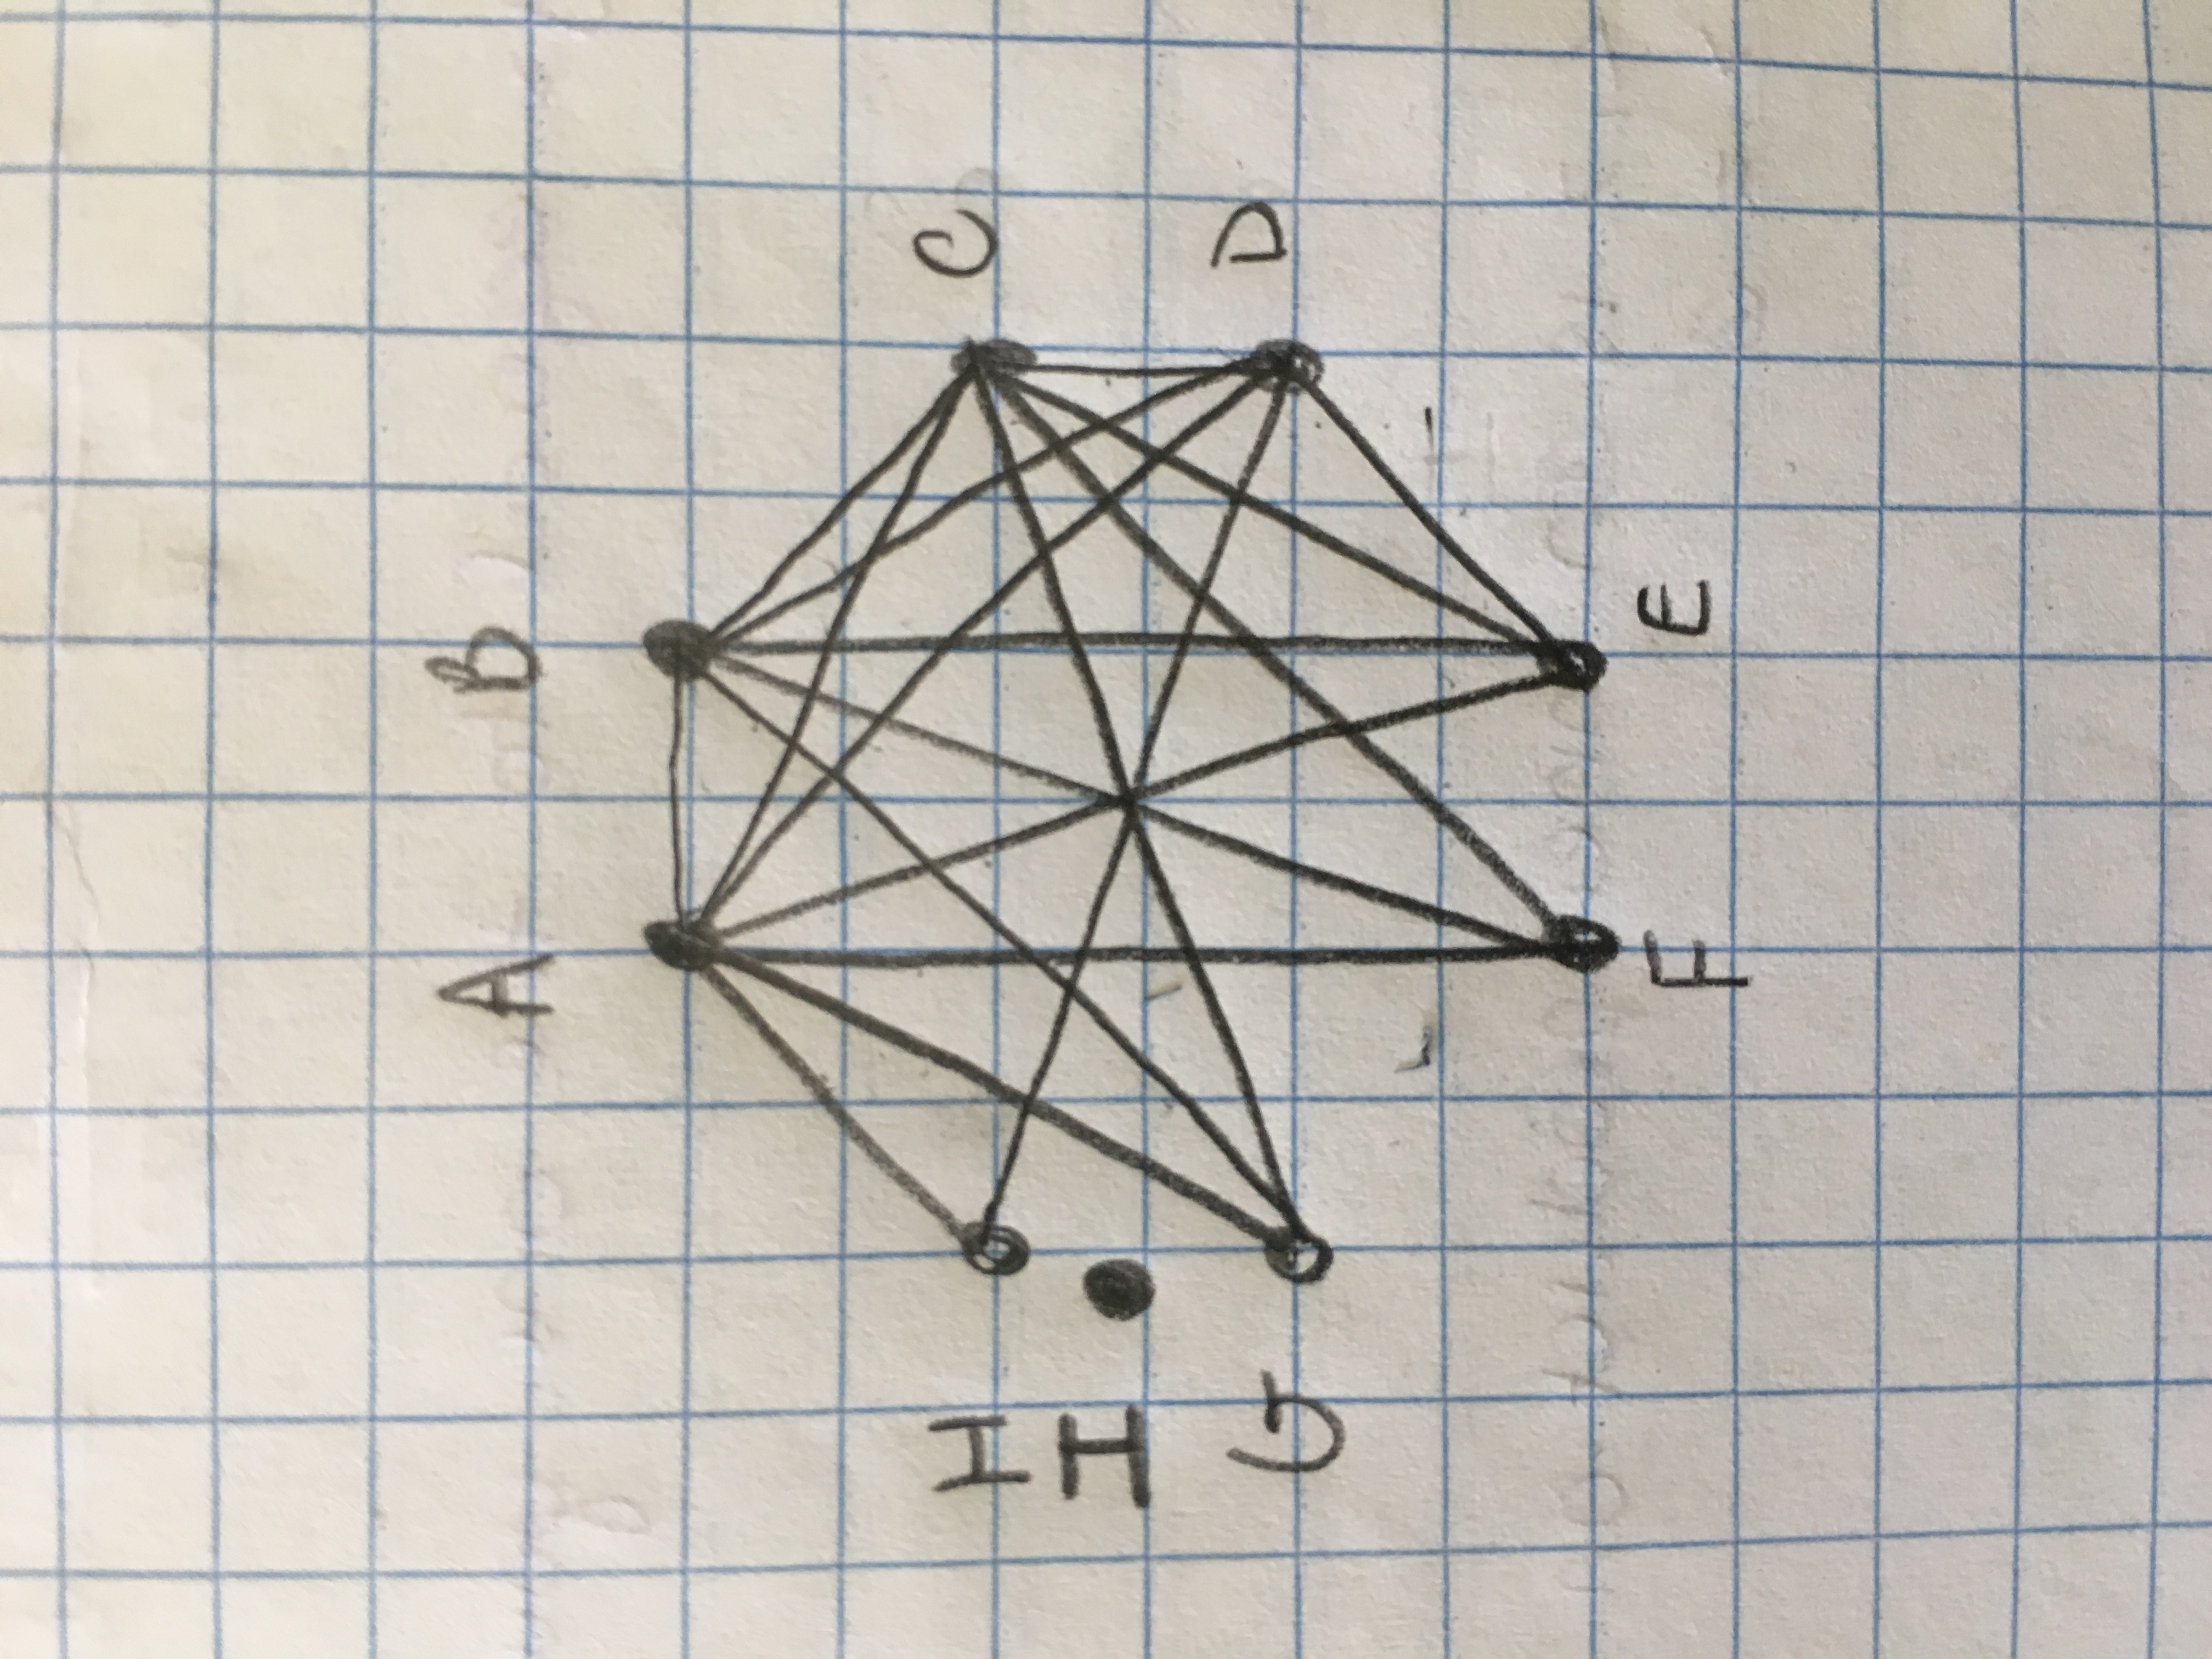
\includegraphics[scale=.05, angle = 270]{IMG_2708.JPG}
    
    \item In a degree sequence with $n$ elements a graph cannot exist if there are vertices with $n-1$ and 0, as one vertex with n-1 requires an edge between it and all other vertices (thus, all other vertices have at least 1 edge). In this degree sequence, there are 9 elements. The first element is 0, and the last is 8 (n-1), thus, this cannot form a graph.
    
    \item In order for a degree sequence to form a graph, there must be an even number of odd vertices (as shown in class). In this degree sequence, there are 5 odd vertices (1, 3, 3, 5, and 7). Therefore, this cannot form a graph.
    
    \item In order for a degree sequence with n elements to form a graph, the sum of the degrees of the n vertices must be less than or equal to $\binom{n}{2}$. As there are 9 elements, the sum of the degrees of all the vertices must be less than or equal to $\frac{9!}{2!7!}$, or 36. The sum of the degrees of the vertices in this degree sequence is $1+2+3+3+4+5+6+8+8$, or 40. As 40 is greater than 36, this degree sequence cannot form a graph.rate
\end{enumerate}

\end{document}
